\section{Qué aportan los índices satelitales}\label{sec:indices}

El reto pregunta qué índice y qué variable climática pesan más. Para responder usamos un bosque aleatorio de análisis,
que aprovecha muchas variables, y medimos cuánto sube su RMSE al revolver los valores de cada índice. Lo hicimos en dos
escenarios (Fig.~\ref{fig:indices}).

\begin{figure}[t]
\centering
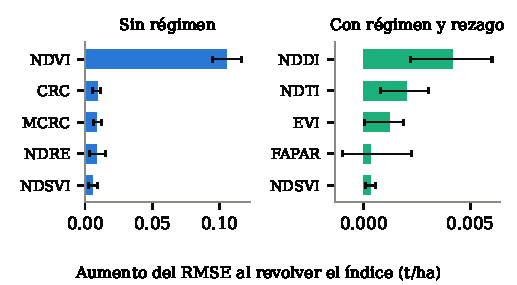
\includegraphics[width=\columnwidth]{f11_indices}
\caption{Aumento del RMSE al revolver cada índice, con su intervalo entre repeticiones. Nótese que las escalas
horizontales son distintas.}
\label{fig:indices}
\end{figure}

Sin el régimen, el NDVI es por mucho el más importante. Revolverlo sube el RMSE 0.106\,t/ha. Pero el NDVI histórico de
cada parcela distingue las zonas y con ellas el régimen, así que en buena parte funciona como un sustituto del
régimen. El modelo solo con variables satelitales llega a 0.696\,t/ha, muy lejos de 0.489 de la media por régimen. Lo
mismo pasa con la lluvia, que sin el régimen sube el RMSE 0.364\,t/ha porque sus celdas de 5\,km identifican la zona.

Con el régimen y el rezago presentes, el índice de sequía NDDI es el que más aporta, pero solo 0.004\,t/ha, y ninguna
variable climática aporta. Es plausible que el NDDI importe, porque marca las parcelas que se secaron o se acamaron
antes en un año muy lluvioso. Aun así, su efecto es mucho menor que el margen de azar de la
Sección~\ref{sec:confiabilidad}. Esta es la razón de fondo por la que el modelo final no usa satélite. Con etiquetas
declaradas y ruidosas, la información de las imágenes queda por debajo del ruido.
